\documentclass[conference,a4paper]{IEEEtran}
\usepackage[T1]{fontenc}
\usepackage{cite}
\usepackage{amsmath,amssymb}
\usepackage{graphicx}
\usepackage{booktabs}
\usepackage{array}
\usepackage{url}
\usepackage{xcolor}
\graphicspath{{../figures/}{figures/}}

% Every number in this file is taken from results/ (see the comment next to it).

\begin{document}

\title{When Does a Learned Latency Model Help\\VNF Placement? A Knowledge-Defined\\Networking Study}

\author{\IEEEauthorblockN{\"Omer Malik Kalemba\c{s}\i}
\IEEEauthorblockA{\textit{Informatics Institute} \\
\textit{Istanbul Technical University}\\
Istanbul, T\"urkiye \\
kalembasi@itu.edu.tr}}

\maketitle

% ---------------------------------------------------------------------------------------------------------------
\begin{abstract}
To place the virtual network functions (VNFs) of a service function chain (SFC), an orchestrator needs to know how
long each VNF will take on each server, but this is usually not observable before the placement is made.
Knowledge-Defined Networking (KDN) proposes to learn such behaviour from network telemetry. We test this idea in a
trace-driven simulation of the 12-node Abilene backbone. Request arrivals and endpoints follow the 2004 Abilene
traffic matrices, and per-request VNF loads come from the public KDN VNF measurement dataset. VNF processing delay
grows with server load, and some servers are secretly slower than others. An XGBoost regressor trained on 170\,559
simulated per-VNF telemetry rows predicts processing delay with $R^2 = 0.997$. A greedy placement method,
\emph{kdn-greedy}, uses these predictions to put each VNF on the server with the lowest predicted path plus
processing delay. Over 30 paired runs at normal load, kdn-greedy reduces the mean end-to-end latency of accepted SFCs, i.e., the
one-way delay of their packets through the chain, by 22\% and 13\% compared with a shortest-path heuristic when
server speeds differ (from 21.5 to 16.8\,ms and from 25.7 to 22.3\,ms), and by 3--4\% when they do not. Near
capacity, where more than half of the requests are rejected, it is up to 3\% slower. This loss comes from optimising
each request on its own, not from prediction error. Replacing the real traffic data with synthetic inputs changes
the gain by at most 0.6\,ms, small next to the 4.6\,ms gain, so the result is driven by the hidden speed
differences between servers, which are an assumption of this study.
\end{abstract}

\begin{IEEEkeywords}
Knowledge-Defined Networking, network function virtualization, VNF placement, service function chaining, machine
learning, XGBoost
\end{IEEEkeywords}

% ---------------------------------------------------------------------------------------------------------------
\section{Introduction}
Network function virtualization (NFV) replaces dedicated middleboxes such as firewalls, NATs and intrusion
detection systems with software VNFs that run on general-purpose servers~\cite{mijumbi2016nfv}. A customer service
is described as a service function chain (SFC): an ordered list of VNFs that the traffic of the service must
traverse~\cite{rfc7665}. When a new SFC is ordered, an orchestrator must choose a server for each VNF. The choice
affects two things: the path the traffic takes through the network, and the time each VNF needs to process the
traffic on the server it runs on.

The placement problem has been studied extensively, with exact integer programs, heuristics and, more recently,
learning-based methods~\cite{herrera2016resource,laghrissi2019survey}. Most formulations assume that the
processing cost of a VNF is known: a constant per VNF type, or a known function of the server load. In a real data
centre this is rarely true. Servers of different hardware generations run side by side~\cite{reiss2012heterogeneity},
and the same workload can run at very different speeds on different machines~\cite{delimitrou2013paragon}. The
orchestrator usually does not know these differences in advance.

Knowledge-Defined Networking (KDN)~\cite{mestres2017kdn}, building on the idea of a knowledge plane for the
Internet~\cite{clark2003knowledge}, proposes a direct answer: the controller collects telemetry from the network,
learns a model of how the network behaves with machine learning, and uses this model to make decisions. This paper
asks a narrow question about that proposal:
\emph{If some servers are secretly slower than others, can a model learned from past per-VNF measurements find
them and place SFCs better than a simple shortest-path rule, and under which load conditions?}

We answer it in a controlled simulation of the Abilene backbone. The contributions are:
\begin{itemize}
\item A trace-driven simulator that combines a real topology, real traffic matrices and real VNF CPU measurements.
We state explicitly which parts are real data and which are our assumptions (Table~\ref{tab:real}).
\item \emph{kdn-greedy}, a placement method that scores every feasible server for every VNF with a learned
processing-delay model plus the known path delay.
\item An evaluation that separates normal operating load from overload. It shows where the gain comes from, how it
depends on server heterogeneity, and why it disappears near capacity.
\item A data ablation showing how much of the result depends on the real traffic data.
\end{itemize}
The code, configuration and all result files are public and every run is deterministic\footnote{\url{https://github.com/kalembasi/traffic-aware-vnf-placement-KDN}}.

\subsection*{Related Work}
\emph{Optimisation-based placement.} VNF-P~\cite{moens2014vnfp} and the work of Bari et al.~\cite{bari2015orchestrating}
formulate VNF placement as an integer linear program and propose heuristics for larger instances. Surveys by
Mijumbi et al.~\cite{mijumbi2016nfv}, Herrera and Botero~\cite{herrera2016resource} and Laghrissi and
Taleb~\cite{laghrissi2019survey} review the many variants of the problem. These methods optimise a cost model that
is given as input; they do not learn it.

\emph{Learning-based placement.} Deep reinforcement learning (DRL) has been used for cluster resource
management~\cite{mao2016deeprm} and for VNF placement in SDN/NFV networks~\cite{pei2020drl}. DRL learns a whole
policy end to end, which can account for future requests but makes it hard to see which piece of knowledge produces
the gain.

\emph{Learning network models.} The KDN line of work learns a model of the network and leaves decisions to a
separate step. Mestres et al.~\cite{mestres2017kdn} predicted the CPU consumption of VNFs from traffic features, and
later studied how well neural networks model network delay~\cite{mestres2018delay}. RouteNet~\cite{rusek2020routenet}
uses a graph neural network to predict per-path delay and uses the predictions to optimise routing.

\emph{Our position.} We do not propose a new optimiser. We follow the KDN split (learn a model, then decide with
a simple search) and measure, in a transparent setting, how much a learned per-VNF delay model is worth for
placement. Hidden server heterogeneity, which motivates scheduling work such as Paragon~\cite{delimitrou2013paragon},
is the knowledge the model is expected to discover.

% ---------------------------------------------------------------------------------------------------------------
\section{Material and Methods}

\begin{table}[t]
\caption{What is real data and what is assumed}
\label{tab:real}
\centering
\footnotesize
\begin{tabular}{@{}>{\raggedright\arraybackslash}p{0.35\columnwidth}>{\raggedright\arraybackslash}p{0.59\columnwidth}@{}}
\toprule
Component & Source and status \\
\midrule
Topology, link delays & SNDlib Abilene~\cite{orlowski2010sndlib}; real (capacities scaled down) \\
Arrival rate over time, ingress/egress & Abilene traffic matrices 2004~\cite{zhang2005anomography}; real, but the
requests themselves are generated \\
Packets and flows of a request, CPU load of its VNFs & KDN VNF dataset~\cite{mestres2017kdn}; real measurements,
borrowed \\
VNF types, chains, CPU/RAM reservations & Our choice (typical literature examples) \\
Processing-delay function & Standard M/M/1 form~\cite{kleinrock1975queueing}; parameters are ours \\
Hidden server speed factors $\kappa_n$ & Our assumption \\
Placements and measured latencies & Simulator output \\
\bottomrule
\end{tabular}
\end{table}

\subsection{Network and traffic}
\emph{Topology.} We use the SNDlib~\cite{orlowski2010sndlib} version of Abilene, a US research backbone with
12 nodes and 15 links (Fig.~\ref{fig:topo}). The propagation delay of a link is the great-circle distance between
its endpoints times 5\,$\mu$s/km (light in fibre). Link capacities are divided by 9.92 (to 1000 and 250\,Mbps) so
that SFC bandwidth demands can saturate links. Each node hosts one server with 100 CPU and 100 RAM units. Traffic is
routed on delay-shortest paths and bandwidth is checked on the chosen path.

\begin{figure}[t]
\centering
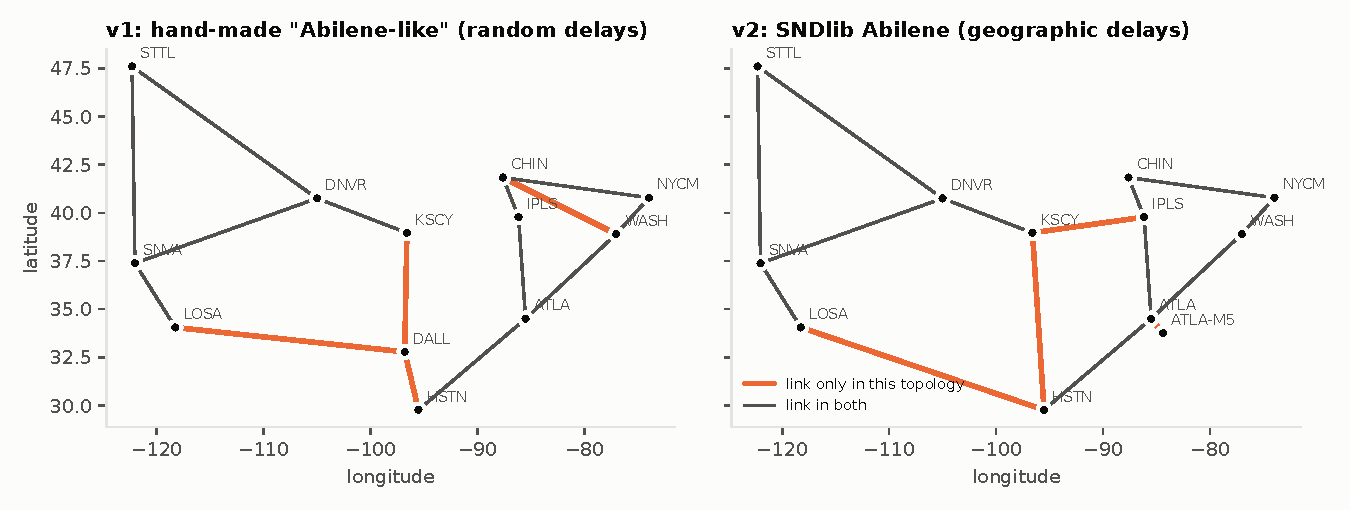
\includegraphics[width=\columnwidth]{fig_topology}
\caption{The SNDlib Abilene topology. Link labels are propagation delays in ms.}
\label{fig:topo}
\end{figure}

\emph{Traffic matrices.} The Abilene traffic matrices~\cite{zhang2005anomography} give, for every 5-minute interval,
the average traffic in Mbps between every pair of the 12 cities, measured with sampled NetFlow. We use the 48\,096
matrices from 1~March to 10~September 2004 (167 of 194 days are present). The data contains only aggregate traffic
volumes: no requests, VNFs, placements or delays. We use it for two things. First, the SFC arrival rate follows the
total traffic volume: requests arrive as a non-homogeneous Poisson process with rate
$\lambda(t) = \lambda \cdot V(t)/\bar V$, where $V(t)$ is the total volume of the current matrix and $\bar V$ its
mean. Second, the ingress and egress of each request are drawn with probability proportional to the current matrix
entry. One 5-minute matrix corresponds to 30 simulation time units (t.u.). March--June is used to generate training
data and July--September for testing.

\emph{SFC requests.} Each request is one of three services, chosen uniformly: Web (NAT$\to$Firewall$\to$Traffic
Monitor, 10\,Mbps), VoIP (NAT$\to$SBC$\to$Firewall$\to$IDS, 20\,Mbps) or Video (NAT$\to$DPI$\to$Video Transcoder,
50\,Mbps). Each VNF type has a fixed CPU and RAM reservation (CPU: 5 for the traffic monitor up to 30 for the video
transcoder). A request lives for a uniformly random 10--600\,t.u.; then its resources are released. A request
models a service order for the aggregate traffic of a customer site, not a single user flow.

\emph{Per-request VNF load.} Mestres et al.~\cite{mestres2017kdn} replayed campus traffic through VNFs (Snort,
a firewall and Open vSwitch) and recorded, for every 20-s traffic batch, 86 traffic features and the CPU
consumption of the VNF. Each request draws one batch, stratified by packet count (Web from the lowest third, VoIP
from the middle third, Video from the top third), and carries the batch's packet and flow counts as observable
traffic features. Each of our VNF types is mapped to the closest measured VNF (NAT and Firewall to the firewall, IDS
and DPI to Snort, the others to Open vSwitch). The relative load $r$ of a VNF is the measured CPU of one of the
5 batches closest in packet count, divided by the median CPU of that VNF. The actual load a VNF adds to its server is
$0.6 \cdot \mathit{cpu}_v \cdot r$, where $\mathit{cpu}_v$ is its reservation. The batches have similar packet counts
(90\% lie between 41\,000 and 59\,000), so $r$ stays within about 0.9--1.1. Admission uses only the reservations;
the actual load is hidden from the controller.

\subsection{Processing delay and hidden server speeds}
The processing delay of VNF $v$ on node $n$ is
\begin{equation}
d_{v,n} = \frac{\kappa_n \, s_v}{1 - \min(\rho_n, 0.95)},
\label{eq:delay}
\end{equation}
the mean sojourn time of an M/M/1 queue~\cite{kleinrock1975queueing}. Here $s_v$ is the base service time of the
VNF (from 0.3\,ms for the traffic monitor to 5\,ms for the video transcoder), $\rho_n$ is the actual load of the
server divided by its capacity, measured after the new SFC is placed, and $\kappa_n$ is a hidden speed factor of
the server. The end-to-end latency of an SFC is the propagation delay of the path ingress$\to$VNF$_1\to\dots\to$
VNF$_k\to$egress plus the sum of the processing delays. It is the one-way delay that every packet of the service
experiences, and it does not depend on how long the service lives.

The speed factors are our assumption, motivated by hardware heterogeneity in real data
centres~\cite{reiss2012heterogeneity,delimitrou2013paragon}. We set $\kappa_n = \exp(\sigma z_{\pi(n)})$, where $z_i$
are the 12 evenly spaced quantiles of the standard normal distribution and $\pi$ is a fixed random permutation of
the nodes. The geometric mean of $\kappa$ is 1 and the same nodes are slow at every $\sigma$. We report two
scenarios: $\sigma = 0$ (all servers equally fast) and $\sigma = 1$ (servers very different, from
$\kappa = 0.18$ in Indianapolis to $\kappa = 5.65$ in Houston). The controller knows the topology and path delays
exactly, but not $r$, $\kappa_n$ or~\eqref{eq:delay}.

\subsection{Learned latency model}
\emph{Telemetry.} We assume per-VNF telemetry: after a placement, the processing delay of each VNF can be measured.
To collect it, we run the simulator on the training months with a randomised placement policy, so that the data
covers many servers at many load levels. For each request it picks uniformly at random one of up to eight heuristic
placements (shortest path with and without load penalties, least-utilised server, co-location at the ingress and
two shuffled first-fit placements). Runs cover $\lambda \in \{0.05, 0.1, 0.2, 0.4\}$ and 20 random seeds, with a
horizon of 10\,000\,t.u. each. Every accepted VNF gives one row; this yields 212\,621 rows per scenario, split by
seed into 170\,559 training and 42\,062 validation rows.

\emph{Features and target.} The model has eight inputs, all observable at decision time: the VNF type and the
host node (one-hot), the measured load of the host before the placement, the CPU this SFC reserves on the host, the
number of this SFC's VNFs on the host, the packet and flow counts of the request, and the mean load of the network.
The target is the processing delay of the VNF. The model does not see $\kappa_n$, but the node identity lets it learn
which servers are slow.

\emph{Model.} We use an XGBoost regressor~\cite{chen2016xgboost} with 150 trees, depth 5 and learning rate 0.1,
trained separately for each scenario. A tree ensemble is a natural choice for tabular data with categorical inputs
and a non-linear response to load.

\subsection{Placement methods}
All methods place the VNFs of a chain one by one, in chain order. A server is \emph{feasible} if it has enough free
CPU and RAM and the link from the previous hop has enough free bandwidth. No method backtracks: if no server is
feasible for some VNF, or the final route to the egress does not fit, the request is rejected.
\begin{itemize}
\item \textbf{greedy} puts each VNF on the first feasible server in a fixed node order. It knows only capacities.
\item \textbf{smart} puts each VNF on the feasible server with the smallest path delay from the previous hop (for
the last VNF, plus the delay to the egress). It knows the topology but nothing about processing.
\item \textbf{kdn-greedy} (ours) scores every feasible server (at most 12) for each VNF: path delay from the
previous hop, plus the predicted processing delay of the VNFs placed so far, including this one, plus the delay to
the egress for the last VNF. Previously placed VNFs are re-scored because co-locating raises the load of their
host. The server with the lowest score wins.
\end{itemize}
As a reference we also run \textbf{oracle-greedy}, the same search with the true processing delay instead of the
prediction. It is the best kdn-greedy could do with a perfect model, not a global optimum.

\subsection{Experimental protocol}
The test runs use July--September 2004, the two scenarios ($\sigma \in \{0, 1\}$) and five arrival rates
$\lambda \in \{0.02, 0.05, 0.1, 0.2, 0.4\}$ requests per t.u. Each $(\sigma, \lambda)$ cell is run with 30 random
seeds for 10\,000\,t.u. (about 28 hours of real traffic), and the first 1\,200\,t.u. are discarded as warm-up. For a
given seed and $\lambda$, all methods see exactly the same request sequence, so differences can be paired by seed.
The primary metric is the mean end-to-end latency of accepted SFCs; we also report the acceptance ratio and the
decision time. Gains are reported as the mean paired difference over the 30 seeds with a 95\% $t$-interval. The
evaluation plan was fixed in a protocol document in the repository before the test runs (see
Section~\ref{sec:discussion} for its history).

Table~\ref{tab:load} shows what each $\lambda$ means for the network. At $\lambda = 0.02$ and 0.05 less than half of
the CPU is reserved on average and at least 96.6\% of the requests are accepted. This is how an operator normally
runs a network: with headroom for peaks and failures, and adding capacity before requests start being refused. At
$\lambda \ge 0.2$ almost every server is full and more than half of the requests are rejected; we treat these levels
as a stress test.

\begin{table}[t]
\caption{Network state at each arrival rate (smart, 30 seeds)}
\label{tab:load}
\centering
\footnotesize
% results/load_levels.md
\begin{tabular}{@{}rrrrl@{}}
\toprule
$\lambda$ & CPU reserved & Full servers$^a$ & Accepted & Regime \\
\midrule
0.02 & 23.3\% & 1.1 of 12 & 99.6\% & normal \\
0.05 & 55.3\% & 4.6 of 12 & 96.6\% & normal \\
0.1  & 81.7\% & 8.9 of 12 & 78.5\% & near capacity \\
0.2  & 92.3\% & 11.1 of 12 & 47.9\% & overload \\
0.4  & 95.6\% & 11.7 of 12 & 27.6\% & overload \\
\bottomrule
\multicolumn{5}{@{}l}{\scriptsize $^a$Free CPU below 30, i.e., cannot host one more video transcoder.}
\end{tabular}
\end{table}

% ---------------------------------------------------------------------------------------------------------------
\section{Experimental Results}

\subsection{Prediction quality}
On the validation rows, the model predicts the per-VNF processing delay with $R^2 = 0.997$ and a mean absolute
error of 0.17\,ms at $\sigma = 1$, about 5\% of the mean delay of 3.2\,ms. At $\sigma = 0$ the values are
$R^2 = 0.999$ and 0.035\,ms (under 2\%). % results/s1/training_metrics.json, results/s0/training_metrics.json
These numbers are high because the target is a noise-free function of observable quantities and the node
identity; the model essentially recovers~\eqref{eq:delay} together with the hidden $\kappa_n$ and the average
load factor. They should not be read as the accuracy one would get on real telemetry. The more relevant question is
how much the predictions improve placement.

\subsection{Latency}
Fig.~\ref{fig:results} and Table~\ref{tab:results} show the mean latency of accepted SFCs.

\begin{figure*}[t]
\centering
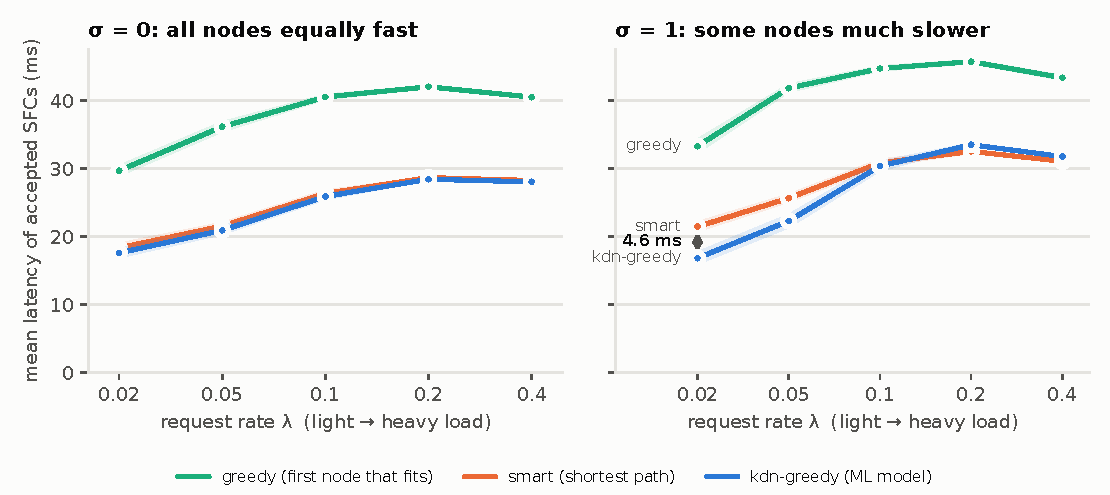
\includegraphics[width=0.82\textwidth]{fig_results}
\caption{Mean end-to-end latency of accepted SFCs, averaged over 30 seeds (shaded bands: 95\% confidence
intervals). Left: all servers equally fast ($\sigma = 0$). Right: some servers much slower ($\sigma = 1$). The two
leftmost points are the normal-load regime of Table~\ref{tab:load}.}
\label{fig:results}
\end{figure*}

\begin{table*}[t]
\caption{Mean latency of accepted SFCs (ms) and gain of kdn-greedy over smart (30 seeds; ms gains are paired
means with 95\% intervals)}
\label{tab:results}
\centering
\footnotesize
% results/paper_tables.md
\begin{tabular}{@{}llrrrrr@{}}
\toprule
Scenario & Method & $\lambda = 0.02$ & 0.05 & 0.1 & 0.2 & 0.4 \\
\midrule
$\sigma = 0$ (equal servers) & greedy & 29.68 & 36.15 & 40.52 & 42.03 & 40.51 \\
 & smart & 18.33 & 21.53 & 26.33 & 28.67 & 28.24 \\
 & kdn-greedy & \textbf{17.59} & \textbf{20.91} & \textbf{25.89} & \textbf{28.43} & \textbf{28.04} \\
 & gain over smart (\%) & $+4.1$ & $+2.9$ & $+1.7$ & $+0.8$ & $+0.7$ \\
 & gain over smart (ms) & $+0.75 \pm 0.09$ & $+0.62 \pm 0.12$ & $+0.45 \pm 0.22$ & $+0.24 \pm 0.20$ & $+0.20 \pm 0.22$ \\
\midrule
$\sigma = 1$ (heterogeneous) & greedy & 33.29 & 41.83 & 44.71 & 45.72 & 43.36 \\
 & smart & 21.45 & 25.65 & 30.82 & \textbf{32.52} & \textbf{31.07} \\
 & kdn-greedy & \textbf{16.82} & \textbf{22.28} & \textbf{30.35} & 33.50 & 31.76 \\
 & gain over smart (\%) & $\mathbf{+21.6}$ & $\mathbf{+13.1}$ & $+1.5$ & $-3.0$ & $-2.2$ \\
 & gain over smart (ms) & $+4.63 \pm 0.36$ & $+3.36 \pm 0.45$ & $+0.47 \pm 0.33$ & $-0.98 \pm 0.26$ & $-0.70 \pm 0.28$ \\
 & seeds won (of 30) & 30 & 30 & 21 & 2 & 6 \\
\bottomrule
\end{tabular}
\end{table*}

\emph{Normal load: the model helps, and more when servers differ.} At $\lambda = 0.02$ and 0.05 with $\sigma = 1$,
kdn-greedy lowers the mean latency by 21.6\% and 13.1\% compared with smart: from 21.45 to 16.82\,ms and from
25.65 to 22.28\,ms (paired gains $4.63 \pm 0.36$ and $3.36 \pm 0.45$\,ms). It is faster in all 30 seeds at both
levels. The slowest requests gain even more: the 95th-percentile latency at $\lambda = 0.02$ drops by 29\%, from
41.9 to 29.7\,ms. With equal servers ($\sigma = 0$) the gain is small but consistent, 4.1\% and 2.9\% (0.75 and
0.62\,ms; 29 of 30 seeds). It comes from the load information in the model: kdn-greedy avoids loaded servers, while smart looks only at
the path. In short, most of the gain comes from finding the hidden slow servers, and the gain grows with how much the
servers differ.

\emph{Near capacity: the gain disappears.} At $\lambda = 0.1$ the gain drops below 2\% (about 0.5\,ms) in both
scenarios. At $\lambda \ge 0.2$ and $\sigma = 1$, kdn-greedy is 2--3\% (0.7--1.0\,ms) slower than smart and loses
in most seeds. The cause
is not prediction error: kdn-greedy is within 0.22\,ms of oracle-greedy in every cell, and in every cell the 95\%
interval of this difference contains zero. The cause is the search itself. kdn-greedy puts every
request on the fastest servers available at that moment; when these fill up, later requests have to use slower or
more distant servers. smart spreads requests along shortest paths and does not create this effect. An oracle that
knows the true delays makes the same mistake, so a better model would not fix it.

\emph{greedy is the worst everywhere.} It ignores paths and sends traffic on long detours: the latency of kdn-greedy is
27--50\% lower than that of greedy (11.6--19.5\,ms) in every cell and every seed. greedy also rejects more requests at medium load
(88.4\% accepted at $\lambda = 0.05$ against 96.6\% for smart).

\emph{Acceptance.} smart and kdn-greedy accept almost the same share of requests at every load (within 1.1
percentage points), so the latency difference is not bought with more rejections.

\subsection{Decision time}
kdn-greedy needs 3.0--8.9\,ms per request on average, against at most 0.37\,ms for smart (Python, one desktop
machine). This cost is paid once per service order, while starting the VNFs themselves takes seconds to minutes and
a service lives for hours or longer. The latency gain, in contrast, applies to every packet for the lifetime of the
service. The decision time matters mainly for scalability: kdn-greedy queries the model for every feasible server,
so it grows linearly with the number of servers.

\subsection{Does the result depend on the real traffic data?}
We repeated the $\sigma = 1$ experiment after removing the real traffic data, one source at a time and both
together (Table~\ref{tab:ablation}). Without the KDN measurements every VNF adds a fixed load ($r = 1$); without the
Abilene matrices requests arrive at a constant rate between uniformly chosen city pairs. To avoid retraining the
model for each variant we used oracle-greedy, which matches kdn-greedy within 0.22\,ms on the original data.

\begin{table}[t]
\caption{Gain over smart (ms) without the real traffic data ($\sigma = 1$, oracle-greedy, 30 seeds)}
\label{tab:ablation}
\centering
\footnotesize
% results/ablation_data.md
\begin{tabular}{@{}lrrrrr@{}}
\toprule
Data used & 0.02 & 0.05 & 0.1 & 0.2 & 0.4 \\
\midrule
Both (original) & 4.63 & 3.39 & 0.41 & $-0.76$ & $-0.81$ \\
No KDN loads ($r = 1$) & 4.46 & 3.20 & 0.26 & $-0.78$ & $-0.62$ \\
No Abilene matrices & 5.01 & 3.31 & $-0.10$ & $-1.10$ & $-0.70$ \\
Neither & 4.85 & 3.15 & $-0.18$ & $-1.04$ & $-0.69$ \\
\bottomrule
\end{tabular}
\end{table}

Removing the KDN loads changes the gain by at most 0.19\,ms; removing the matrices as well changes it by at most
0.58\,ms. Both are small next to the gain itself (4.63\,ms at $\lambda = 0.02$). At normal load and at overload the sign of the result is the same in every row; only at $\lambda = 0.1$,
where the gain is small anyway, does it change sign. The gain is therefore
determined by the hidden server speeds and the distances in the topology, not by the traffic data. The real data
makes the request stream realistic, but it does not carry the result.

% ---------------------------------------------------------------------------------------------------------------
\section{Conclusion (Future Work)}
We tested the central KDN idea, learning network behaviour from telemetry and using it for decisions, on VNF
placement in a controlled simulation of the Abilene backbone. A learned per-VNF delay model combined with a simple
greedy search finds hidden slow servers and lowers the mean SFC latency by 13--22\% (3.4--4.6\,ms) compared with a
shortest-path heuristic at normal operating load. The gain shrinks to 3--4\% when all servers are equally
fast, and it disappears near capacity, where placing every request on the currently best servers hurts later
requests. The answer to our question is therefore: a learned latency model helps when there is hidden, learnable
variation between servers and the network has headroom.

Future work follows from the limitations below. First, the method should be trained and tested on real per-VNF
telemetry, where measurements are noisy and the delay does not follow a known formula. Second, near capacity the
placement has to account for future requests; combining the learned delay model with a load-balancing term or with
reinforcement learning~\cite{pei2020drl} is a natural next step. Third, the model should be updated online as servers
and traffic change, and the evaluation should be extended to larger topologies and to VNF sharing between services.

% ---------------------------------------------------------------------------------------------------------------
\section{Discussion}
\label{sec:discussion}
\emph{What the study shows and what it does not.} None of the datasets contains VNF placements or latency
measurements. Latencies are computed by the simulator from~\eqref{eq:delay}, and the slow servers are placed there
by us. The study therefore does not show that machine learning lowers latency in a real network. It shows that if
there is a hidden but learnable difference between servers, a model trained on telemetry can find it and use it, and
it measures how large the benefit is under different loads. The size of the gain depends directly on this assumption:
3--4\% without heterogeneity, 13--22\% with strong heterogeneity.

\emph{Why the prediction is so accurate.} An $R^2$ of 0.997 is a property of the simulator, not of the model:
the target has no noise. Real telemetry would add measurement noise, interference between co-located VNFs and
effects that no feature captures. Both the prediction accuracy and the placement gain would likely be lower.

\emph{The role of the real data.} The ablation shows that the real traffic matrices and VNF measurements change the
gain by less than 0.6\,ms, against a gain of up to 4.6\,ms. The packet counts in the KDN dataset are similar to each other, so the load factor $r$
varies by only about $\pm$10\%. We keep the data because it gives the simulator a realistic request stream and a
measured relation between traffic and CPU load, but the paper should not be read as a result about these datasets.

\emph{Overload.} The loss at $\lambda \ge 0.2$ is a limitation of per-request greedy optimisation, shared by the
oracle. In practice an operator does not run a network in this regime, where more than half of the orders are
refused; the remedy there is more capacity, not a better placement rule.

\emph{Other limitations.} We use a single 12-node topology, one server per node, and a separate VNF instance for every
request (no sharing or scaling of VNFs). The model is trained once and never updated. The processing-delay form is
a simple queueing model with parameters chosen by us. The decision times were measured in Python and indicate an
order of magnitude only.

\emph{Design history.} The evaluation protocol in the repository was registered before the data was generated. In its
first version, the model only selected among the (up to eight) heuristic placements also used to collect telemetry. Because these candidates were
generated without knowledge of the server speeds, they rarely contained a placement that avoided the slow servers.
The gain over smart was smaller at every load and negative from $\lambda = 0.1$ on. kdn-greedy, in which the model builds the placement itself, was
added to the protocol after these results were known and before it was run. The repository contains the first
version and further variants (other baselines, intermediate $\sigma$ values, a different delay form); they are not
needed for the conclusions of this paper.

\emph{Reproducibility.} The full pipeline (data download, simulation, training, tables and figures) runs with a
single script in about 30 minutes on 12 cores. All runs use fixed seeds and every number in this paper is taken from
a result file in the repository; only the decision times vary between runs.

% ---------------------------------------------------------------------------------------------------------------
\section*{Acknowledgements}
I thank my advisor Tu\u{g}\c{c}e Bilen for the guidance throughout this seminar, and the maintainers of SNDlib and
the authors of the KDN datasets for making their data public.

\bibliographystyle{IEEEtran}
\bibliography{refs}

\end{document}
